\section{2015-05-29 Product Manager Interview}

\textbf{Todd:} Thank you. 00:01

\textbf{Interviewee:} Yes. You're welcome. 00:02

\textbf{Todd:} I was hoping you could describe your typical day. 00:04

\textbf{Interviewee:} My typical day, okay. We start every morning with stand up. It takes about five minutes. And that's where we go over what we did yesterday or what we're going to do today, any blockers or anything like that. I think the format differs from project to project but usually that's how I like to do it. 00:24

\textbf{Interviewee:} Then, I'll go through emails just to have some alone time and just go through my emails and things like that. And if I'm working with a client PM, we will then start going through the backlog. We might pair on writing stories. We might prioritize the backlog. 00:44

\textbf{Interviewee:} Usually, during the beginning of the week, we'll have an iteration planning meeting. It takes an hour and that's where we'll go through and go over some of the stories we've prioritized in the backlog and the dev will then point them or estimate them. 01:03

\textbf{Todd:} Thank you. Anything else? 01:08

\textbf{Interviewee:} There's more of the same stuff. There's lunch and then I might have a meeting or two sometimes just some internal sort of product meeting. All the PMs might meet once a week, once every other week or something like that. 01:22

\textbf{Todd:} We all say we do iterative development. For your perspective, what makes us iterative? 01:29

\textbf{Interviewee:} What makes us iterative is that we don't fully flush out a feature or anything like that upfront. And so we just take a first pass at it and get the basic functionality of it down and then layer on  top of that. 01:48

\textbf{Interviewee:} We might add some improvements or we may add some styling or we might add different things like that but we don't do that all upfront. Now, we can just get something workable  done. 02:02

\textbf{Interviewee:} Ideally, in front of users usually by that point, we're not, in the beginning, we're not putting anything in front of production or anything like that but that's the idea. We potentially could, which I think makes it iterative. 02:16

\textbf{Todd:} Thank you. This is my first drawing exercise for you. So, pretty open-ended question, could you describe a project work flow by drawing it on that sheet of paper? There's no wrong answers. 02:32

\begin{figure}[h]
\centering
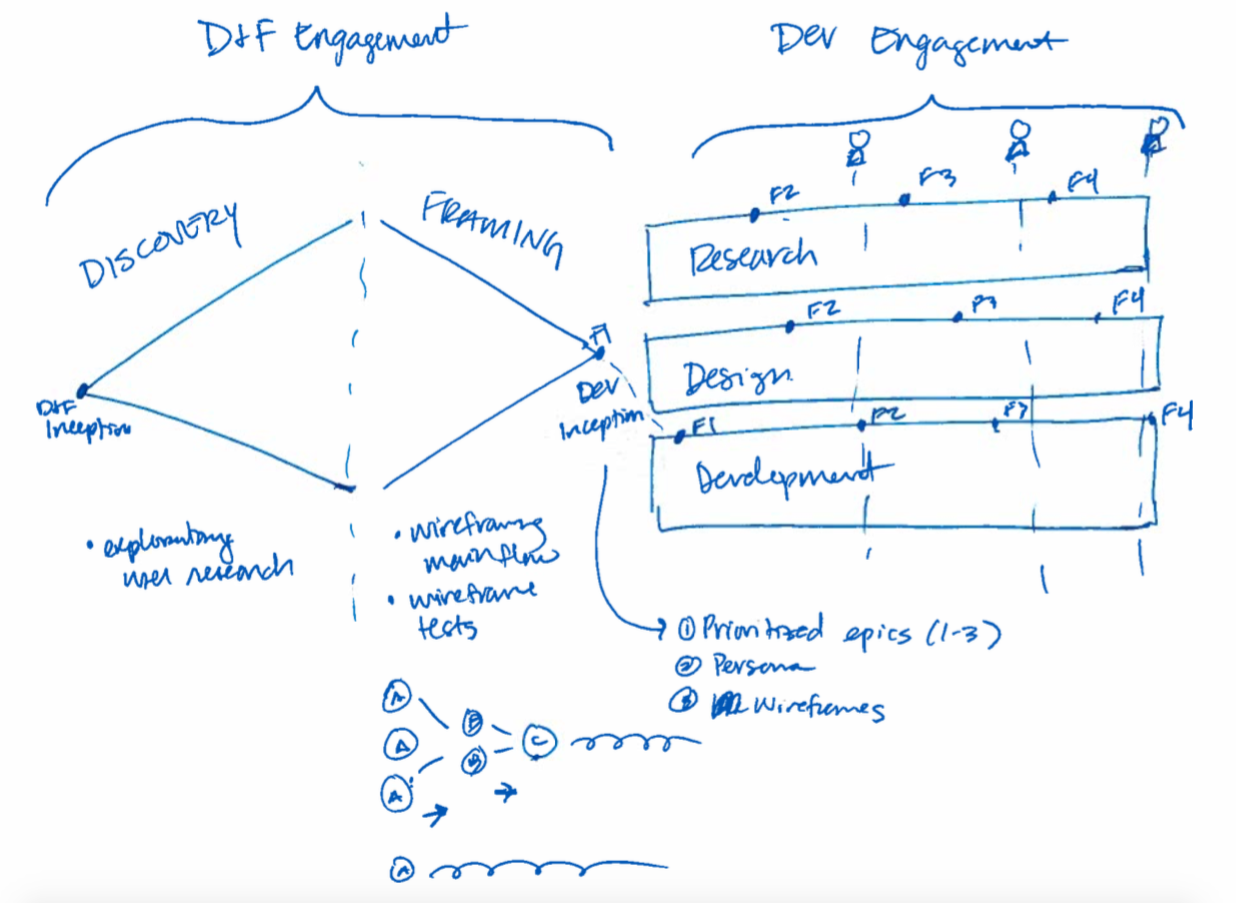
\includegraphics[width=6.5in]{interviews/2015_05_29.png}
\caption{\quotes{2015-05-29's drawing of a project work flow}}
\label{2015_05_29}
\end{figure}

\textbf{Interviewee:} Does it matter if there's a DNF first or...? 02:39

\textbf{Todd:} However you want it. Typical, ideal, however you want to draw it. 02:44

\textbf{Interviewee:} We actually show this to clients. We have this drawing here. 02:54

\textbf{Interviewee:} Most of the projects that I've been on start with the DNF. We'll call this DNF. 03:07

\textbf{Interviewee:} It's assuming the project has design in development going. This kind of, like, inception. 03:27

\textbf{Interviewee:} And this is dev inception. 03:32

\textbf{Interviewee:} This is your discovery, and framing. 03:50

\textbf{Interviewee:} Here in this area, we're sort of doing more exploratory research and sort of going wide trying to understand the users. That's something we do at the beginning of every project especially if the client doesn't know who their user is or they have ideas of who they are but it's not validated. 04:10

\textbf{Todd:} 	That's the discovery phase. 04:11

\textbf{Interviewee:} Yes. So, this is like exploratory user research. That's like interviews and maybe on site, shadowing people and things like that. And once we have a good idea of who they are, we start wire framing, maybe like the main flow and doing some wire frame tests like user research, that kind of thing and that's kind of within that, I think, we're kind of iterating as well. 04:45

\textbf{Interviewee:} I guess you can either start with one and iterate on that or you can start with many and narrow down. We've done both. So, when you start with many, you just- So, this is like your different As, research, then research to get to C. That makes sense? 05:10

\textbf{Todd:} It's like a portfolio of ideas? 05:14

\textbf{Interviewee:} Yes. I did it on my first project and it worked out really well and then from there you're kind of iterating on what you've come up with. 05:25

\textbf{Interviewee:} We came up with a couple, different nuance ways of doing something because they all seem good and they're like, two or three different features and we sort of combined them in different ways and then we took our insights from that and narrowed it down two versions, narrowed it down to one version. 05:46

\textbf{Interviewee:} I've also done it where you just start with A and you just iterate. I think both worked but this is fun to do. By the time we get to dev inception, we have prioritized epics. You have a develop persona. And you have wire frames. That's kind of the ideal for this point. At that point, development can start on say feature one and in the meantime, we'll start researching feature two. Then, we'll develop it. Then, feature three. So, it kind of goes like that. 06:37

\textbf{Todd:} Nice. 06:39

\textbf{Interviewee:} Maybe you have feature one here and then we'll go here. While they're doing that, we'll start on the next thing. So, on the next thing it flows down. I hate saying waterfall because I know it's the wrong kind. It's like a different kind of waterfall but it iterates in that way. So, we're like, \quotes{Oh, it's going in the cycle.} At any time, we're going to bring in users to test whatever we want. 07:09

\textbf{Todd:} You're drawing people. 07:12

\textbf{Interviewee:} Yes. These are users. At any given point, we can even do exploratory research. We can do wire frame or visual research or we can show them an actual prototype. 	It's kind of nice because you can, whenever you need people, whenever you're stuck on something, you don't have to wait for the right time to bring people in. 	It's just you can test anything at any given time.  07:34

\textbf{Todd:} Thank you. Have you seen a project that didn't quite fit this, what you've drawn here, this model? Or it was really different? 07:46

\textbf{Interviewee:} Yes. I was on a project. I was only on it for two weeks. It was just really quick enablement but there's basically no DNF. They came in with full visuals, full design. The problem is not a lot of it was validated. A lot of it was like, \quotes{Oh, the stakeholders thing. This looks nice.} 08:02

\textbf{Interviewee:} That was kind of different. As a PM, it was weird to write stories for full visual designs because I wasn't sure where to draw the line with the styling and things like that. We kind of had to feel it out. I think we stopped at colors and 	fonts. 	08:19

\textbf{Interviewee:} We did colors, fonts and a little bit of spacing for some other things but no animations, nothing like that. And that's also hard to convince the client, that maybe this isn't the right solution or things like that. I'm not sure how they got 	through without validation but it happens sometimes. 08:43

\textbf{Todd:} Do you think because it had such detailed mocks, they were married to their ideas? 08:49

\textbf{Interviewee:} I think so. It wasn't too hard, they're actually pretty open minded about stuff because they trust at our process. A lot of clients come in and like, \quotes{We trust you.} 08:58

\textbf{Interviewee:} For the most part, all the projects I've been on have been very flexible from that standpoint but I definitely felt bad for making the designer go through stuff. I don't think he minded but it's just a little bit harder to push back on things when they're not black and white and flexible. 09:21

\textbf{Todd:} Can you think of a different project that maybe didn't fit this mold in a different way? 09:27

\textbf{Interviewee:} Not out of the ones I've been on. They've mostly followed this. Like my first project followed this to a T. It was great. The second one just didn't have any discovery or framing. Right now, we kind of follow this as well. 09:51

\textbf{Todd:} I think given our sales process, we set this up for us. 09:56

\textbf{Interviewee:} You mean like non labs projects. 10:02

\textbf{Todd:} Just some labs. 10:02

\textbf{Interviewee:} 	Oh, just some labs. 10:03

\textbf{Todd:} Or in Pivotal. 10:06

\textbf{Interviewee:} Yeah. I haven't heard of any that- I think there are some enterprise projects that this doesn't quite work because there's an added QA layer. I haven't worked with a QA team but it just makes it harder to follow this because there's a QA layer that you have to go through in addition to acceptance. 10:28

\textbf{Todd:} In my current project, there's an approval process on designs and they want to see everything. You can't really do the features incrementally at least on design level. 10:40

\textbf{Interviewee:} That sucks. We have some design reviews. On most of the projects I've been on, we had weekly design reviews so nothing was a huge surprise to people. I guess I've just gotten lucky with the clients. They've been mostly receptive to our process. I hear horror stories about it but I haven't personally experienced any huge ones just yet. 11:09

\textbf{Todd:} As a PM, it feels like there's a lot that you juggle and manage. Is there one or two things that you remind yourself each day? What's the most important thing that you try to get right on a project? 11:26

\textbf{Interviewee:} If I'm working with a client, I always have to think about what I'm going to do with them. I think that's the biggest worry because I think any of the stuff I can do myself really quickly and I'll just remember things as they come up but I have to remember that I have to enable the client. 11:42

\textbf{Interviewee:} I have to be cognizant of what are we going to do today? What does the week look like? Not just the PM but I think PM in design especially during this period. It really helps to plan out the week just roughly and figure out okay, when are we doing research? What are some activities we should do? 12:01

\textbf{Interviewee:} There's some things you have to think about with the client from their perspective. Maybe they're not open to something. How do I convince them that this is the right way and try to put myself in their shoes and have empathy for them so I know how I can help turn them around to something that can work. Or help them come up with the idea. And I'm just like, \quotes{Oh you came up with this idea.} That kind of thing. 12:29

\textbf{Todd:} You mean you had the idea and you helped them realize the idea as well? Is that what you were saying? 12:35

\textbf{Interviewee:} Yes. We wanted them to go a certain way but they were like, \quotes{No we have to go this way.} How can we make them think that they came up with going this way. 12:43

\textbf{Todd:} It's like inception. You plant seeds. 12:45

\textbf{Interviewee:} Yes because they only listen to you so much. You tell people, \quotes{Trust me.} But they'll only trust you so much and then when they actually experience it, sometimes you just have to let people make a mistake and they feel that pain and they're like, \quotes{Oh okay. I will never do that again.} maybe not do that again maybe try this way. \quotes{Let's see what happens with that.} It's shows a different way of thinking. 13:12

\textbf{Todd:} What's it, for instance, on letting the client make a mistake and letting them feel that? 13:17

\textbf{Interviewee:} One time we had some clients who were very, very tight to us that are features and they call them core capabilities and very concrete and final and we kept trying to say, \quotes{Okay. These are assumptions.} They just didn't understand the word assumption. They're like, \quotes{No. We need to build these things.} 13:34

\textbf{Interviewee:} So, we did a couple of rounds of research because they weren't down for research. They never done that before and once they heard certain things, I think even though they heard certain things, their brain was still telling them they want these core capabilities. So, it's like they were, what is that called, like a confirmation bias or something like that or they're just like, \quotes{Oh yeah. That's what it means.} 13:53

\textbf{Interviewee:} And so, we did a synthesis and mapped out everything out and took their core capabilities and our main insights and tried to match them up. I think from there we could see that a lot of the insights didn't map to the core capabilities but it wasn't aggressive. We were all doing it together. 14:12

\textbf{Interviewee:} They were the ones making the mappings and saying like, \quotes{Oh. This moves down in priority. We didn't expect this to come up. Let's move on this first.} It took more time but it was nice that they came up with those conclusions on their own in a way or able to see that rather than us just telling them don't worry about this. Focus on the research. 14:37

\textbf{Interviewee:} You have to remember these clients come up with these things for months or years so they're very tied to them and to just rip them away from that is insensitive. I can empathize with them. You just have to have slowly validate or invalidate the stuff that they've been so closely tied to. 14:58

\textbf{Todd:} You described the client relationship and the parties you have with that. When you think about the development team, I'm biased, how to set them up for success, what's sort of things do you try and enable or set up for the team? 15:13

\textbf{Interviewee:} For the developers specifically? 15:15

\textbf{Todd:} PM. They're trying to make everything hum than what you imagine. 15:19

\textbf{Interviewee:} I keep communication really open. Before I start a project, if I can I like to talk to whoever is the anchor or the designer in the team and just get a feel for how they work with the PM because everybody's a bit different. 15:36

\textbf{Interviewee:} Big things that they would expect from a PM that I might miss or something like that and just try to get a feel for how they work with other people and obviously retro is great for a lot of that stuff. 15:50

\textbf{Interviewee:} Sometimes, we've had retros where we just talk about- because I think in front of the client you have to have a united front. And for the most part, in my experience, it's been great but if there are any disagreements or any problems, you don't want to bring up in front of the client it's really nice to have a pivotal retro. 16:09

\textbf{Todd:} How frequently might you have one of those? 16:12

\textbf{Interviewee:} Depending on how bad the project is. Once a week, maybe. Maybe once every other week. I don't know. 16:19

\textbf{Todd:} On top of the normal retro? 16:21

\textbf{Interviewee:} On top of. We have the normal retro usually and if we were at a point where we're feeling disconnected, we might have one. So, it kind of depends. I've never been in a situation where I needed one weekly. Although I've heard of those, really stressful ones. 16:39

\textbf{Todd:} Think of one of the worst projects you've been on, what's one thing you did to try and right it and get it back on track? 16:47

\textbf{Interviewee:} I haven't had any that were horrible. I think there was some bad times in my first project because the client wasn't committing to certain things. Once they went back to their own office. 17:10

\textbf{Interviewee:} We're working remotely and they were just being pulled into meetings. I think I was a little harsh. I don't know. I was just like, \quotes{Hey, the backlogs' drying, designing guys need to do stuff.} Because the devs were running out of things to do. They're just like, \quotes{What do we do?} 17:27

\textbf{Interviewee:} I tried to find other things that didn't require design to be prioritized. For that, I needed some help from the anchor because I don't have a formal technical background. 17:39

\textbf{Interviewee:} A lot of times I'll just ask. I'm like, \quotes{Hey, teach me this stuff.} Sometimes I'll have the devs say in stand-up that the backlogs' dry because I find the people listen to devs more than PMs or they take it more seriously. So, I'm just like, \quotes{Okay. You just say it.} I can say it 10 times but as soon as the devs say it, they're like, \quotes{Oh my god. [Interviewee] We're freaking out.} And I was just like, \quotes{Yes. I was freaking out two weeks ago.} 18:09

\textbf{Interviewee:} Sometimes you just have to be a little harsh. Just be like, \quotes{I know you have a meeting but we really need to move on this right now.} 18:21

\textbf{Interviewee:} I also paired with devs and designers which I think helped bring the team a little bit closer. The client PM was there half the time but I encourage him to pair sometimes. I really like cross functional pairing. 18:35

\textbf{Todd:} When you pair with dev, do you work on a story with the dev?18:39

\textbf{Interviewee:} Yes. I do whatever they're doing and I'm not necessarily coding from scratch but I know enough to recognize where things go. We'll type this in here or I might watch them do something then I'll do it. 18:52

\textbf{Interviewee:} A lot of it is discussion and asking questions. Like on this particular time, I had been on a project longer than the dev and so she wasn't sure where everything lived and I was like, \quotes{I think that data is over here. Can we do control+F for this keyboard} We're trying to figure out why something didn't work and I had a little more context so I was able to talk about it and she's like, \quotes{Oh. I know where that is. Let's try doing that type of thing.} It was a lot of back and forth. 19:22

\textbf{Todd:} Nice. I have not experienced that. 19:25

\textbf{Interviewee:} Yes. It's really fun. I love pairing with devs. It's also really intimidating. If you're at the helm of a spaceship or something and you're just like, \quotes{Oh my god.} but it's pretty fun. Everybody I've paired with has been really nice and patient and they like teaching. I was like, \quotes{Cool. Teach me.} 19:41

\textbf{Todd:} Pairing with designers makes sense to me, I think. 19:48

\textbf{Interviewee:} Yes. Again, it's a lot of discussion. Maybe we should put this here instead of there. I didn't know how to use Illustrator before but know I can poke around and use it. So, sometimes I get to do some stuff too. 20:01

\textbf{Todd:} That's fantastic. 20:03

\textbf{Interviewee:} Yes, it's really fun. 20:04

\textbf{Todd:} So, as a dev, sometimes I think about non functional requirement or they're called quality attributes. How do you handle those? As a PM, how does that work for you? Do you think about them? 20:19

\textbf{Interviewee:} You mean like visual design, thing like that? 20:23

\textbf{Todd:} Things like maybe performance or security or liability of the system. We call them ilities. There's like 20 of them that might show up in a project. 20:31

\textbf{Interviewee:} Yes. I think about them a little bit, honestly, in my experience here, at least. It's usually the devs or the client PM who is bringing it up. I should think about it more probably but when I think about MVP, it's like user mode but I think those get prioritized. 20:49

\textbf{Interviewee:} We just feel it out and honestly it's more of the client PM's decision and because they know the product better. If they're really, really lost, we'll try to make the most informed decision with them. 21:02

\textbf{Interviewee:} If we're about to launch or we want to do an initial release and obviously some of that stuff has to go forward. If some things, like really unknown or there's high risk, sometimes we try to write a story and just get that one story out there because that drives out a lot of the risk and drives out a lot of things that we might not know. 21:21

\textbf{Todd:} Trying to reduce risk makes sense to me. In my experience at Pivotal, I've not seen any stories about performance or things like that. That makes sense at some level because stories are about features. They're not about attributes of the system and I haven't seen how anyone here handles that. I'm curious... 21:44

\textbf{Interviewee:} I try to write all stories from a user perspective so I might say something like, \quotes{I want the spatial load faster because it's taking a really long time right now.} That kind of thing and so I know some places have requirements of loads in two seconds and things like that. 22:01

\textbf{Interviewee:} I haven't quite gotten down to that level but I'll still write it from a user perspective and if I have an idea of what might be slowing something down for example, I'll put it in there. \quotes{Oh, we have a page full of SVGs maybe we can convert them on to PNGs or something like that.} I try not to be too prescriptive because that's just not my place. 22:24

\textbf{Todd:} Good. 22:27

\textbf{Interviewee:} I try to handle them from the user perspective as much as possible. 22:30

\textbf{Todd:} I have created a little model for stories. This is now called described or something. Defined. 22:44

\textbf{Todd:} From your perspective, this is a flow of stories, give me feedback for me on those. 22:53

\textbf{Interviewee:} Named is just identifying the story. Once you flush them out and written them and they've been through pre-IPM and they're estimated, they're started, blocked. I usually don't go back and estimate. So, it's like this. 23:12

\textbf{Todd:} It could happen. 23:13

\textbf{Interviewee:} I usually don't do this. I guess it depends on what's happening here. I haven't re-estimated a story unless we pointed it five weeks past and then it comes up in the backlog, we might revisit it and say, \quotes{Okay. Do we still think it re-points?.} 23:35

\textbf{Todd:} Well, we try not to re-point. I agree with that. 23:37

\textbf{Interviewee:} I haven't done that. Started, finished, delivered, accepted. 23:42

\textbf{Interviewee:} Delivered. Checked in. This would go back to - Oh, you have that here. Delivered. So, when will it go from delivered to started?  23:56

\textbf{Todd:} The irony is this actually comes form tracker data, this graph. I went through a ton of project and watched all the transitions of every story and there was a story from delivered to started. 24:08

\textbf{Interviewee:} Maybe they delivered on accident? That sometimes happens. Or was it delivered on purpose? 24:14

\textbf{Todd:} I think what happens there is you deliver it and then you realize there's more work to be done. 24:19

\textbf{Interviewee:} Oh, so the dev will go back and... 24:20

\textbf{Todd:} Say, \quotes{Oops. We're not done.} 24:23

\textbf{Interviewee:} Okay. 24:24

\textbf{Todd:} Or someone will walk by and say, \quotes{That's not done. You didn't do X.} 24:28

\textbf{Interviewee:} Just like  before the PM hits something, they'll say, \quotes{Hey, you guys, forgot this.} 24:32

\textbf{Todd:} It's kind of like the rejection where the PM didn't reject it. 24:34

\textbf{Interviewee:} That makes sense. I've done that before. Finish, delivered, accepted. 24:40

\textbf{Todd:} That has happened, believe it or not. 24:47

\textbf{Interviewee:} Really? 24:48

\textbf{Todd:} I agree with you, the ideal is that would not happen. My point in showing this is to actually help you make sense of what I'm about to show you next. This is my view of stories. 24:56

\textbf{Interviewee:} I've been trying to create a checklist items for each state that the story could go in. I just wanted you to look at this list and see if you have any... 25:06

\textbf{Interviewee:} The idea is, for something to be named how do you know it's named or not and these would have to happen for each state. If this is not clear, ask questions and I'll try and clarify. 25:19

\textbf{Interviewee:} Okay. I think this is like an either/or. It could be prioritized or it could not be. Can we write down? 25:34

\textbf{Todd:} Sure. Whatever you want. 25:36

\textbf{Interviewee:} Defined. Feature is prioritized. I think this can also be either/or. 25:45

\textbf{Interviewee:} I usually don't prioritize until - I'll have a rough priority but I'll wait until they're all flushed out. Sometimes in pre-IPM even they're not fully prioritized by this time. Usually after they're estimated, usually they're prioritized but sometimes after they estimate, I'll rethink some things. 26:13

\textbf{Interviewee:} If they're not fully prioritized, that's okay. 26:16

\textbf{Interviewee:} Story describes clear acceptance criteria. That makes sense. That makes sense. 26:22

\textbf{Interviewee:} Story only describes user interaction with system. Yes. I think some people do this. I really like to do this. Oh, ideal PM. 26:33

\textbf{Todd:} That's your ideal. 26:34

\textbf{Interviewee:} Yes. 26:35

\textbf{Todd:} It doesn't have to happen. 26:35

\textbf{Interviewee:} Yes. Business value is clear. Yes. I'd say, relevant. Did you already write that? 26:59

\textbf{Todd:} No. I did not. 26:59

\textbf{Interviewee:} I try to attach design to every story. I try not to write a story before a design is done and that works out really well. And that's kind of the ideal. 27:09

\textbf{Interviewee:} Estimated. Feature is estimated. Nothing blocks developers from working on the story. Yes. I would even make this required. 27:24

\textbf{Todd:} I've estimated stories that were blocked that's why it's ideal. So you feel strongly about that. 27:34

\textbf{Interviewee:} If it's blocked, I don't. 27:36

\textbf{Todd:} Why do you estimate it? 27:37

\textbf{Interviewee:} It's not going to be accurate. I guess there are some stories where the devs are kind of like, \quotes{Well, I've never worked with that before.} If something's not defined or this is clearly blocked then I'll probably be like, \quotes{Okay. We'll just wait.} 28:00

\textbf{Todd:} Would you say it would be okay to estimate if you're trying to figure out when the end of the project is going to be even though things might be blocked? 28:06

\textbf{Interviewee:} Yes. I can see doing that. I've heard of that. I haven't don that on a project yet but I know they've been pointing  parties where people do small, medium, large type of thing or really rough pointing estimates. I think that's fine but for an IPM when you're going to work on something ideally, it's not blocked. Started. Yes. Blocked. It depends to you. Yes. I think that makes sense. I can't speak to these two. 28:37

\textbf{Todd:} You've paired on code so you might have more of an opinion on that than other PMs. 28:45

\textbf{Interviewee:} I agree with it. It makes sense. It was funny, I was pairing with somebody and we were working on an iOS project but it also involved JAVA and so we had, was it C\# or not C\#, what is it? 28:58

\textbf{Todd:} Objective C. 28:59

\textbf{Interviewee:} I guess she's more familiar with Objective C and not JAVA. She's kind of like, \quotes{Oh. I don't know Java that much.} She was like, \quotes{It all looks the same to me.} It looks equally confusing. 29:15

\textbf{Interviewee:} Units test pass, makes sense. Acceptance passes. What is the difference between a unit test and acceptance test? 29:28

\textbf{Todd:} Unit test are the very low level. They test one thing in isolation. Acceptance test, they're more PM level. Does the feature do what it's supposed to do? Does the story work? 29:42

\textbf{Interviewee:} So, the devs will do an acceptance test. 29:47

\textbf{Todd:} Sometimes they have them sometimes they don't it depends on the project so I'll probably put ideal or optional on there as well. 29:51

\textbf{Interviewee:} Is that something actually written or is that more of like the devs going through what they acceptance criteria says? 30:02

\textbf{Todd:} It depends on the project. Some of them we will write acceptance test. 30:08

\textbf{Interviewee:} Code reviewed prior to commit. Changes reviewed prior to commit. That makes sense. Delivered. Yes. PM updated the acceptance criteria because they were not clear. 30:28

\textbf{Todd:} You're going to fill out some of these. Go ahead keep going. 30:32

\textbf{Interviewee:} I do some of these things. Additional requirements that need to be implemented. The PM changed the requirements and the codes need rework. This shouldn't happen. This shouldn't happen. This shouldn't happen. 30:50

\textbf{Todd:} I completely agree with you. 30:52

\textbf{Interviewee:} If the PM changes their requirements, if it's small, sometimes, I'll say, \quotes{I meant this but I forgot to put it in.} If it's really tiny, they're like, \quotes{It's okay we'll just do it.} I'm like, \quotes{Okay. Thanks} 31:03

\textbf{Todd:} Why write another story. 31:03

\textbf{Interviewee:} Yes. And I'll just put a comment. I'll say, \quotes{It works but I forgot to add this.} So, devs rejecting so you can add this thing or something like that. But if it's something big, I'll be like, \quotes{Sorry, I forgot that.} And I'll just write another story. I'll be like, \quotes{Let me just write another story.} 31:23

\textbf{Interviewee:} Sometimes I'll write a bug and I don't have a clear criteria when it's a bug and when it's an extra feature but in the moment it makes sense. I just can't think what I used to decide it's a bug or not. 31:38

\textbf{Todd:} I know what I use. 31:43

\textbf{Interviewee:} One time, we were building something where you can adjust the quantity in a card and we were like, \quotes{It has to be an integer. it can't be zero.} And we were able to add zero and we were like, \quotes{We shouldn't be able to add zero.} That was a rejection but the fix they made, it had to be applied to this other scenario that wasn't covered in the story. But since they did it for one, \quotes{Okay. Let's just create a bug for it.} Because it was treated as a bug in the other scenario so it's kind of like a weird scenario. 32:21

\textbf{Todd:} For me, the black and white description is, if the story says it should do something and the code doesn't, that's a bug. If a story doesn't describe that condition, then it's a new feature. 32:32

\textbf{Interviewee:} Yes. 32:34

\textbf{Todd:} There's probably a gray area. 32:36

\textbf{Interviewee:} Yes. There are some gray areas where you decide should I reject it or should I write a bug type of thing. I think, definitely, in that first scenario, it's either reject a bug or usually that would just be a rejection because it says it should do this but it doesn't. 32:49

\textbf{Interviewee:} Anything additional should be another story but sometimes I do a bug instead of a rejection for some reason and I think it's for little things. PM updated the acceptance criteria because they're not clear. That sometimes happens. If it's small. So, I'll say, if it's small. And sometimes when I reject something if it's really nitpicky, I'll put nit. Do you guys do that? 33:18

\textbf{Todd:} What does that mean for you? 33:21

\textbf{Interviewee:} I don't know. A dev told me to do that one. I think it stands for nitpicky or nitpicking. I don't know. Sometimes, I'll be like the word is off or something. Technically it can go out but it should have this other word or the color is a little bit wrong and I'm just this works perfectly but I'll say it, nit. 33:44

\textbf{Todd:} So, in the comments of the story, you will put nit:fix this. 33:51

\textbf{Interviewee:} Yes. I feel it's a little nicer. I don't know. It's just like nothing's wrong, it's just the mock has this and it's a UI type of thing. A Dev told me to do that once. I was like, \quotes{Okay. I feel better about doing that because I feel bad rejecting stories that are technically work but just have a weird...} 34:10

\textbf{Todd:} I think I've seen one PM not accept it and put a comment on it,  which notifies people and then they would accept it once it's fixed. But rejection is probably the right flow. 34:22

\textbf{Interviewee:} Yes. If it's not rejected, you're not going to see it. As a dev, I would imagine. QA manager added new requirements. This should happen. I just think that's so silly but I guess some big companies have a QA process but they should not add new requirements. They should be bugs features and then... 34:55

\textbf{Interviewee:} I've had QA say, \quotes{Oh, this doesn't work.} or \quotes{This has this one case it won't take a credit card after 2049.} I was just like, \quotes{Okay. Let's write a bug} but I just put at the bottom backlog. We'll put them in the backlog but the PM will prioritize it as they prioritize everything else. That shouldn't lead to a rejection ever. 35:17

\textbf{Todd:} Given everything that we talked about in this conversation, is there anything else that you think would be relevant? Maybe questions I should ask? 35:26

\textbf{Interviewee:} What is your objective? What stuff do you want to know? 35:31

\textbf{Todd:} I should have a clear answer to that question. I think at this point, I'm really curious how what we do differs from what Kent Beck described 15 years ago. We've done a lot of really neat things and so I've been really interested in that. And I have a question I'd prefer to ask without leading it. Why do we call an IPM an iteration planning meeting? 36:10

\textbf{Interviewee:} Versus? 36:13

\textbf{Todd:} Why do we call it that? There's things that we do in the meeting and does the name describe what we do in the meeting? What's the purpose of an IPM? 36:27

\textbf{Interviewee:} It's so the team is aligned in what we're going to be doing for the next iteration or the next week. I guess, sometimes, the things that you point in IPM don't always line up to what you're going to be working on in a week. Sometimes, we'll end up pointing a lot of things. I think it's a good way. I think ideally, it is supposed to spell what the team is going to be working on for the next week or the next iteration. 36:54

\textbf{Interviewee:} So, you know you have immediate contact. You just pointed it. You know exactly what's happening. There's not a lot of time between for you to forget. Most of the time it happens or at least you'll start working on some of the things you pointed on that week but I think also it's a good rhythm setter for the team like you meet every week and you feel like you have this check in. You're always connected. You have frequent connections with dev and PM and design. Because I think PM and design can be off. We're usually ahead, design especially but PM, kind of split but we have fear what's going on right now and also be two weeks ahead and so I feel like this helps bridge the gap between what's going on in the design world and the dev world and having those check ins really helps 37:48

\textbf{Todd:} For me, it's like weekly estimation meeting. About six months into my career here, I realized that, for me, in my perspective there is no iteration. We do retros on Fridays because Mondays we don't remember what we did last week. We do weekly estimation meetings somewhere in the middle because we need to have enough work. The worst thing that could probably happen is I have six devs with nothing to do. So, we need to make sure that there's enough of a backlog for them. I was on a project where I had no idea that iteration started on Tuesday. And that was the clue for me. What? Are there iterations starting on Tuesday? I had no idea. 38:28

\textbf{Interviewee:} So, what do iterations mean for you then? 38:31

\textbf{Todd:} I think there is no spoon. I think it's a very kanban-like the work flows through us. The team isn't committing to a scrum that says, next week we're going to deliver these three features. 38:44

\textbf{Interviewee:} Yes. I can see what you mean by that. I feel that way, too, sometimes. 38:49

\textbf{Todd:} I think that's great. We show up and we do where the work is needed. 38:54

\textbf{Interviewee:} Yes. 38:56

\textbf{Todd:} So, halfway through a week something in the universe completely changes, we respond to it and start adapting to it. It's not like there's this ready plan. On Friday, we're going to launch this feature. We can't do that. In the original definition of XP, the team was committing to where they will be each week. 39:16

\textbf{Interviewee:} I didn't know that. 39:17

\textbf{Todd:} Yes. 39:18

\textbf{Interviewee:} I had no idea. I thought XP was totally. 39:21

\textbf{Todd:} And you couldn't change what the team would do that week? It was inflexible. 39:24

\textbf{Interviewee:} That's against everything that we do. I actually didn't know that and I read the XP book. 39:30

\textbf{Todd:} If the PM changed what they did during the first week, there was a contract violation between you and the team. 39:36

\textbf{Interviewee:} That's so crazy. I need to go re-read that book or something because I totally have been telling clients XP is flexible. 39:41

\textbf{Todd:} and..with XP..what we do here. That's really interesting. 39:45

\textbf{Interviewee:} Yes. That's kind of how I see it. I think, if anything, it gives a team a rhythm. I think retros help us sort of figure out what didn't go well during the week. What we need to change so it's not at some arbitrary point somebody might say, \quotes{This isn't working. Let's try to figure out how to change it} There's a forced check in so anything that you think you had a problem with this week, you know we'll come up at least every week and then you can do something to make the next week better. I think, work flow wise, maybe we're not doing things iteratively but team-cadence wise, we have iterations of like, Okay. Let's take an arbitrary piece of time. A day's too short, a month is too long. So, let's do a week. Just make sure there are teams running smoothly every week. I think it serves that purpose maybe more than the actual delivery and execution. It's more about the team spirit, I guess. 40:59

\textbf{Todd:} I think what I'm hearing you say is, your view of the word iteration might be different than mine and so you're happy to call in IPM because, for you, it's this weekly rhythm that's maybe artificial because of weekends. If there were no weekends, we might have a different rhythm or something 41:20

\textbf{Interviewee:} Yes. 41:21

\textbf{Todd:} It wouldn't be healthy 41:22

\textbf{Interviewee:} Yes. I think it's like a force check in because we were just to do things. We think about things in terms of time and so if we didn't have a time marker I think we would just get very confused and we would get very lost in what we're doing. 41:40

\textbf{Interviewee:} And even new devs are estimating stories, they still want to estimate in terms of time. We're always thinking in terms of time because that's how the world works in a way and so I think having that time marker helps us keep things in check versus if we just let them run on forever. 41:58

\textbf{Interviewee:} So, yes. I guess I think about iterations. I haven't thought about this deeply before but I guess me, for iterations, it's more like the team rhythm and team cadence versus the actual execution of things. 42:09

\textbf{Todd:} Yes. Okay. 42:11

\textbf{Interviewee:} I guess iteration in context of how we use it here. 42:14

\textbf{Todd:} That's very helpful for me. I'll have to deep think on it some more. 42:18

\textbf{Interviewee:} Building iteratively I think it means something else. Like what I was saying in the beginning, you just start with the first layer and the second layer. That's a little bit different than what I'm thinking in terms of team iteration if that makes sense. 42:31

\textbf{Todd:} It does. I don't have anything else. Is there anything else you wanted to share or anything you're not telling me? 42:40

\textbf{Interviewee:} I don't think so. I've worked in waterfall before so this is like a huge breath of fresh air. I think it's much healthier. I think the ideal of what this is supposed to be is good but it's not always applicable especially with enterprises, for example. We've definitely had to bend a little bit more to work with enterprises because it's just not the solution for everybody. You have to cater a little bit to different types of organizations. 43:19

\textbf{Todd:} I forgot about demographics. How long have you been at Pivotal? 43:21

\textbf{Interviewee:} I've been here almost a year. I started in August. 43:25

\textbf{Todd:} Just in terms of your career, when did you graduate from college? 43:31

\textbf{Interviewee:} 2010. 43:32

\textbf{Todd:} Great. That's it. 43:33

\textbf{Interviewee:} Okay. Cool. 43:34

\textbf{Todd:} Thank you. 43:34

\textbf{Interviewee:} Yes. Thank you. This was fun. 43:36

